% !TeX root = ../main.tex
\graphicspath{{Figures/Results}}

\chapter{Results}\label{ch:results}

\section{Model Performance}\label{results:sec:model_perf}

\begin{itemize}
  \item \textbf{Objective:} What task is being evaluated here, and on what dataset?
  \item \textbf{Baseline:} What is the model being compared against?
  \item \textbf{Roadmap:} What metrics will be shown to support that the model works?
\end{itemize}


\subsection{Sensitivity}
\begin{enumerate}
  \item \textbf{Context and Visual:} Re-states why the test was run and points immediately to the corresponding graphic. - "To evaluate [biological metric], [analytical tool/pipeline] was executed, revealing [general pattern] (Figure X)."
  \item \textbf{High-Level Takeaway:} States the primary finding cleanly in plain English. - "[Feature A] demonstrated a [direction] correlation with [Feature B], modifying [metric] by [value] fold ([Statistical test identifier], [degrees of freedom] = [value], p = [value])."
  \item \textbf{Core Evidence:} Backs up the takeaway using exact metrics, stats, and values. - combined above
  \item \textbf{Resolution / Boundary:} Highlights the limits, outlier sequences, or edge cases. - "Conversely, this trend was absent in [Sub-population/Cluster X], which maintained an unchanged baseline value of [Value]."
\end{enumerate}




\begin{figure}[H]
  \centering
  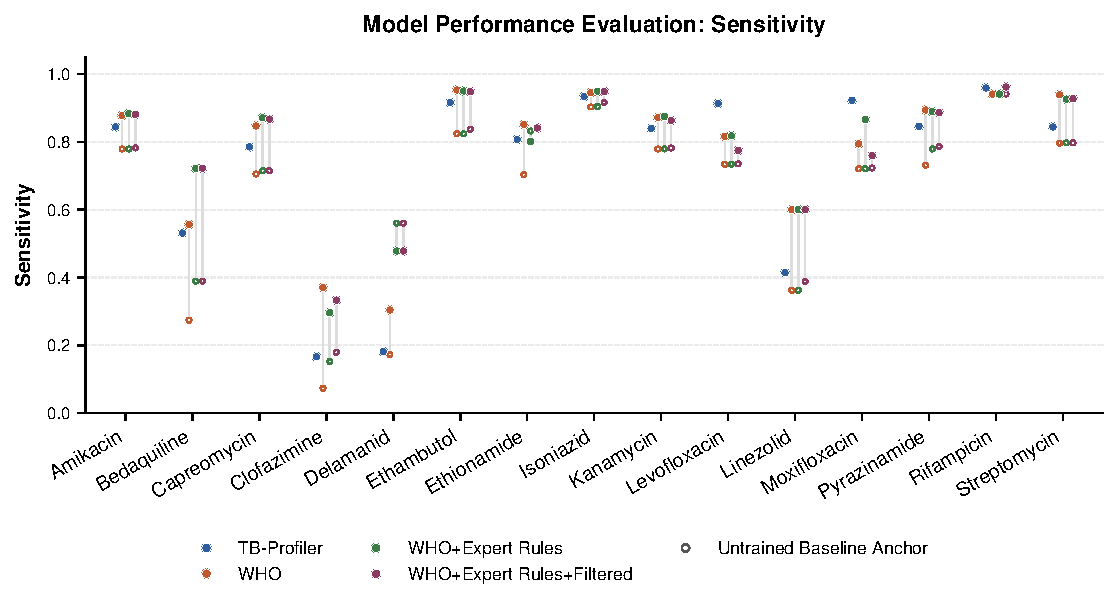
\includegraphics[width=\textwidth]{figures/sensitivity.pdf}
  \caption{Sensitivity of the neural network with tb-profiler as the baseline, WHO, and WHO augmented with
  expert rules, and filtered is shown aswell. The naive pass with only the catalogues encoded as 1s , or 0s
  is shown as empty circles, and the trained model results are filled in.}\label{fig:sens}
\end{figure}

\subsection{Specificity}

\begin{figure}[H]
  \begin{center}
    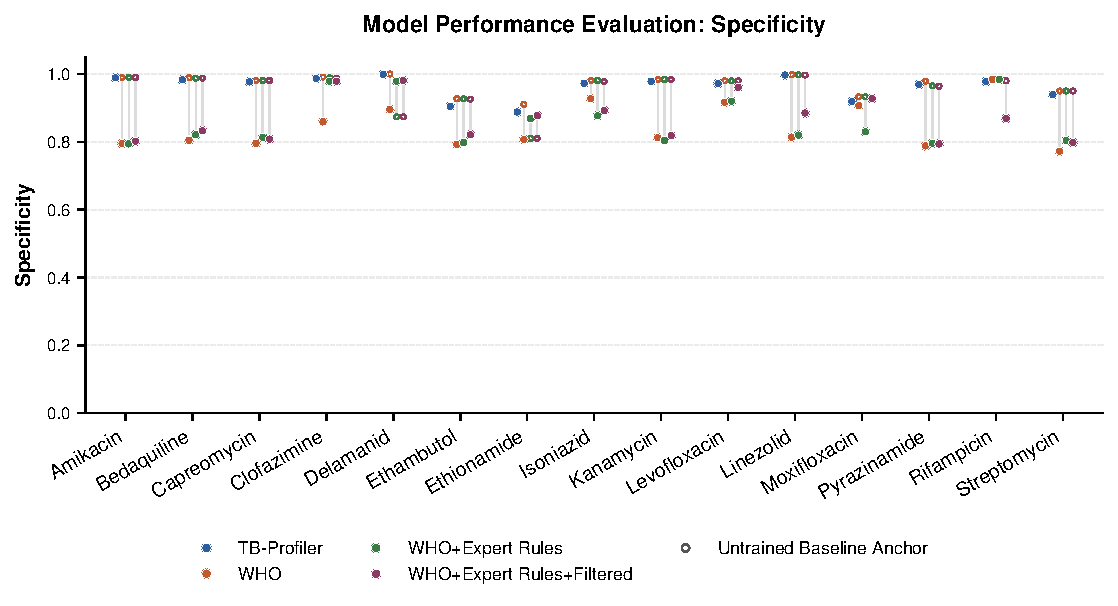
\includegraphics[width=\textwidth]{figures/specificity.pdf}
  \end{center}
  \caption{Specificity of the neural network after training for 15 Anti-TB drugs that had at final confidence
  grading of 1 or 2. TB-profiler (blue) acts as the baseline to show how the neural networks perform with different
  weights. Weights were constructed from the WHO catalogue, and then augmented with expert rules and filtered snps.
  These are represented as hollow circles, and after training, they are represented as filled circles.}\label{fig:spec}
\end{figure}

\subsection{F1 Score}

\begin{figure}[H]
  \begin{center}
    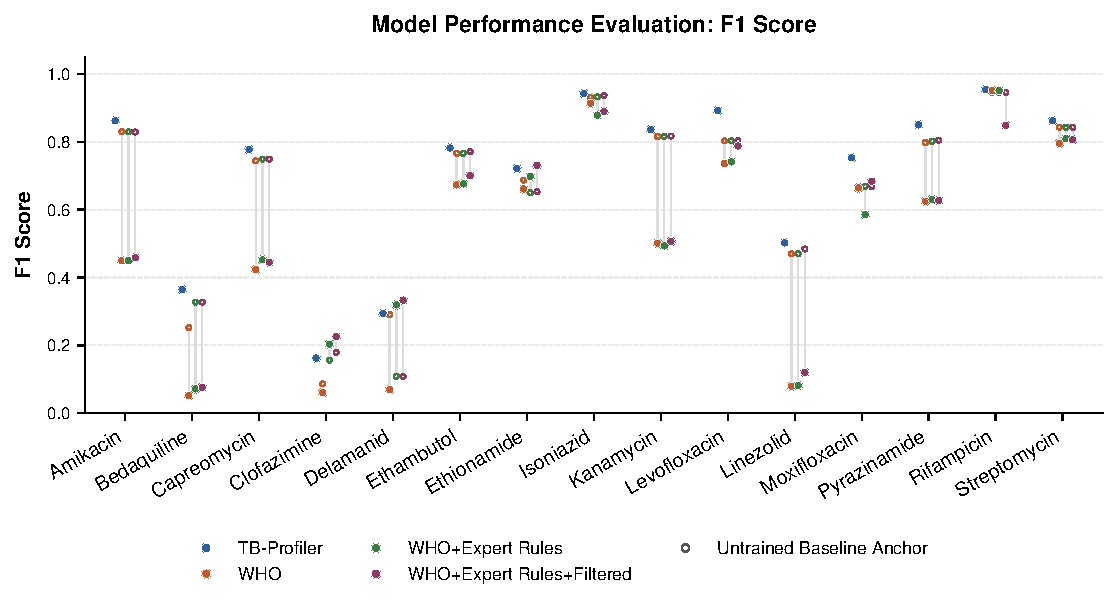
\includegraphics[width=\textwidth]{figures/f1.pdf}
  \end{center}
  \caption{F1 scores of the neural networks, with F1 being the balanced average between specificity and sensitivity.
  In this plot, TB-profiler is used as a baseline, colored in blue, and the untrained networks with shown with hollow
  circles. The trained models are shown with filled circles.}\label{fig:f1}
\end{figure}

\subsection{Training and Efficiency}

\section{Candidate Mutations}
\begin{itemize}
  \item \textbf{Objective:} What task is being evaluated here, and on what dataset?
  \item \textbf{Baseline:} What is the model being compared against?
  \item \textbf{Roadmap:} What metrics will be shown to support that the model works?
\end{itemize}
\subsection{First-line Drugs}

\subsection{Second-line Drugs}

\subsubsection{Group A}

\subsubsection{Group B}

\subsubsection{Group C}

\subsection{Other drugs}

\begin{figure}[H]
  \begin{center}
    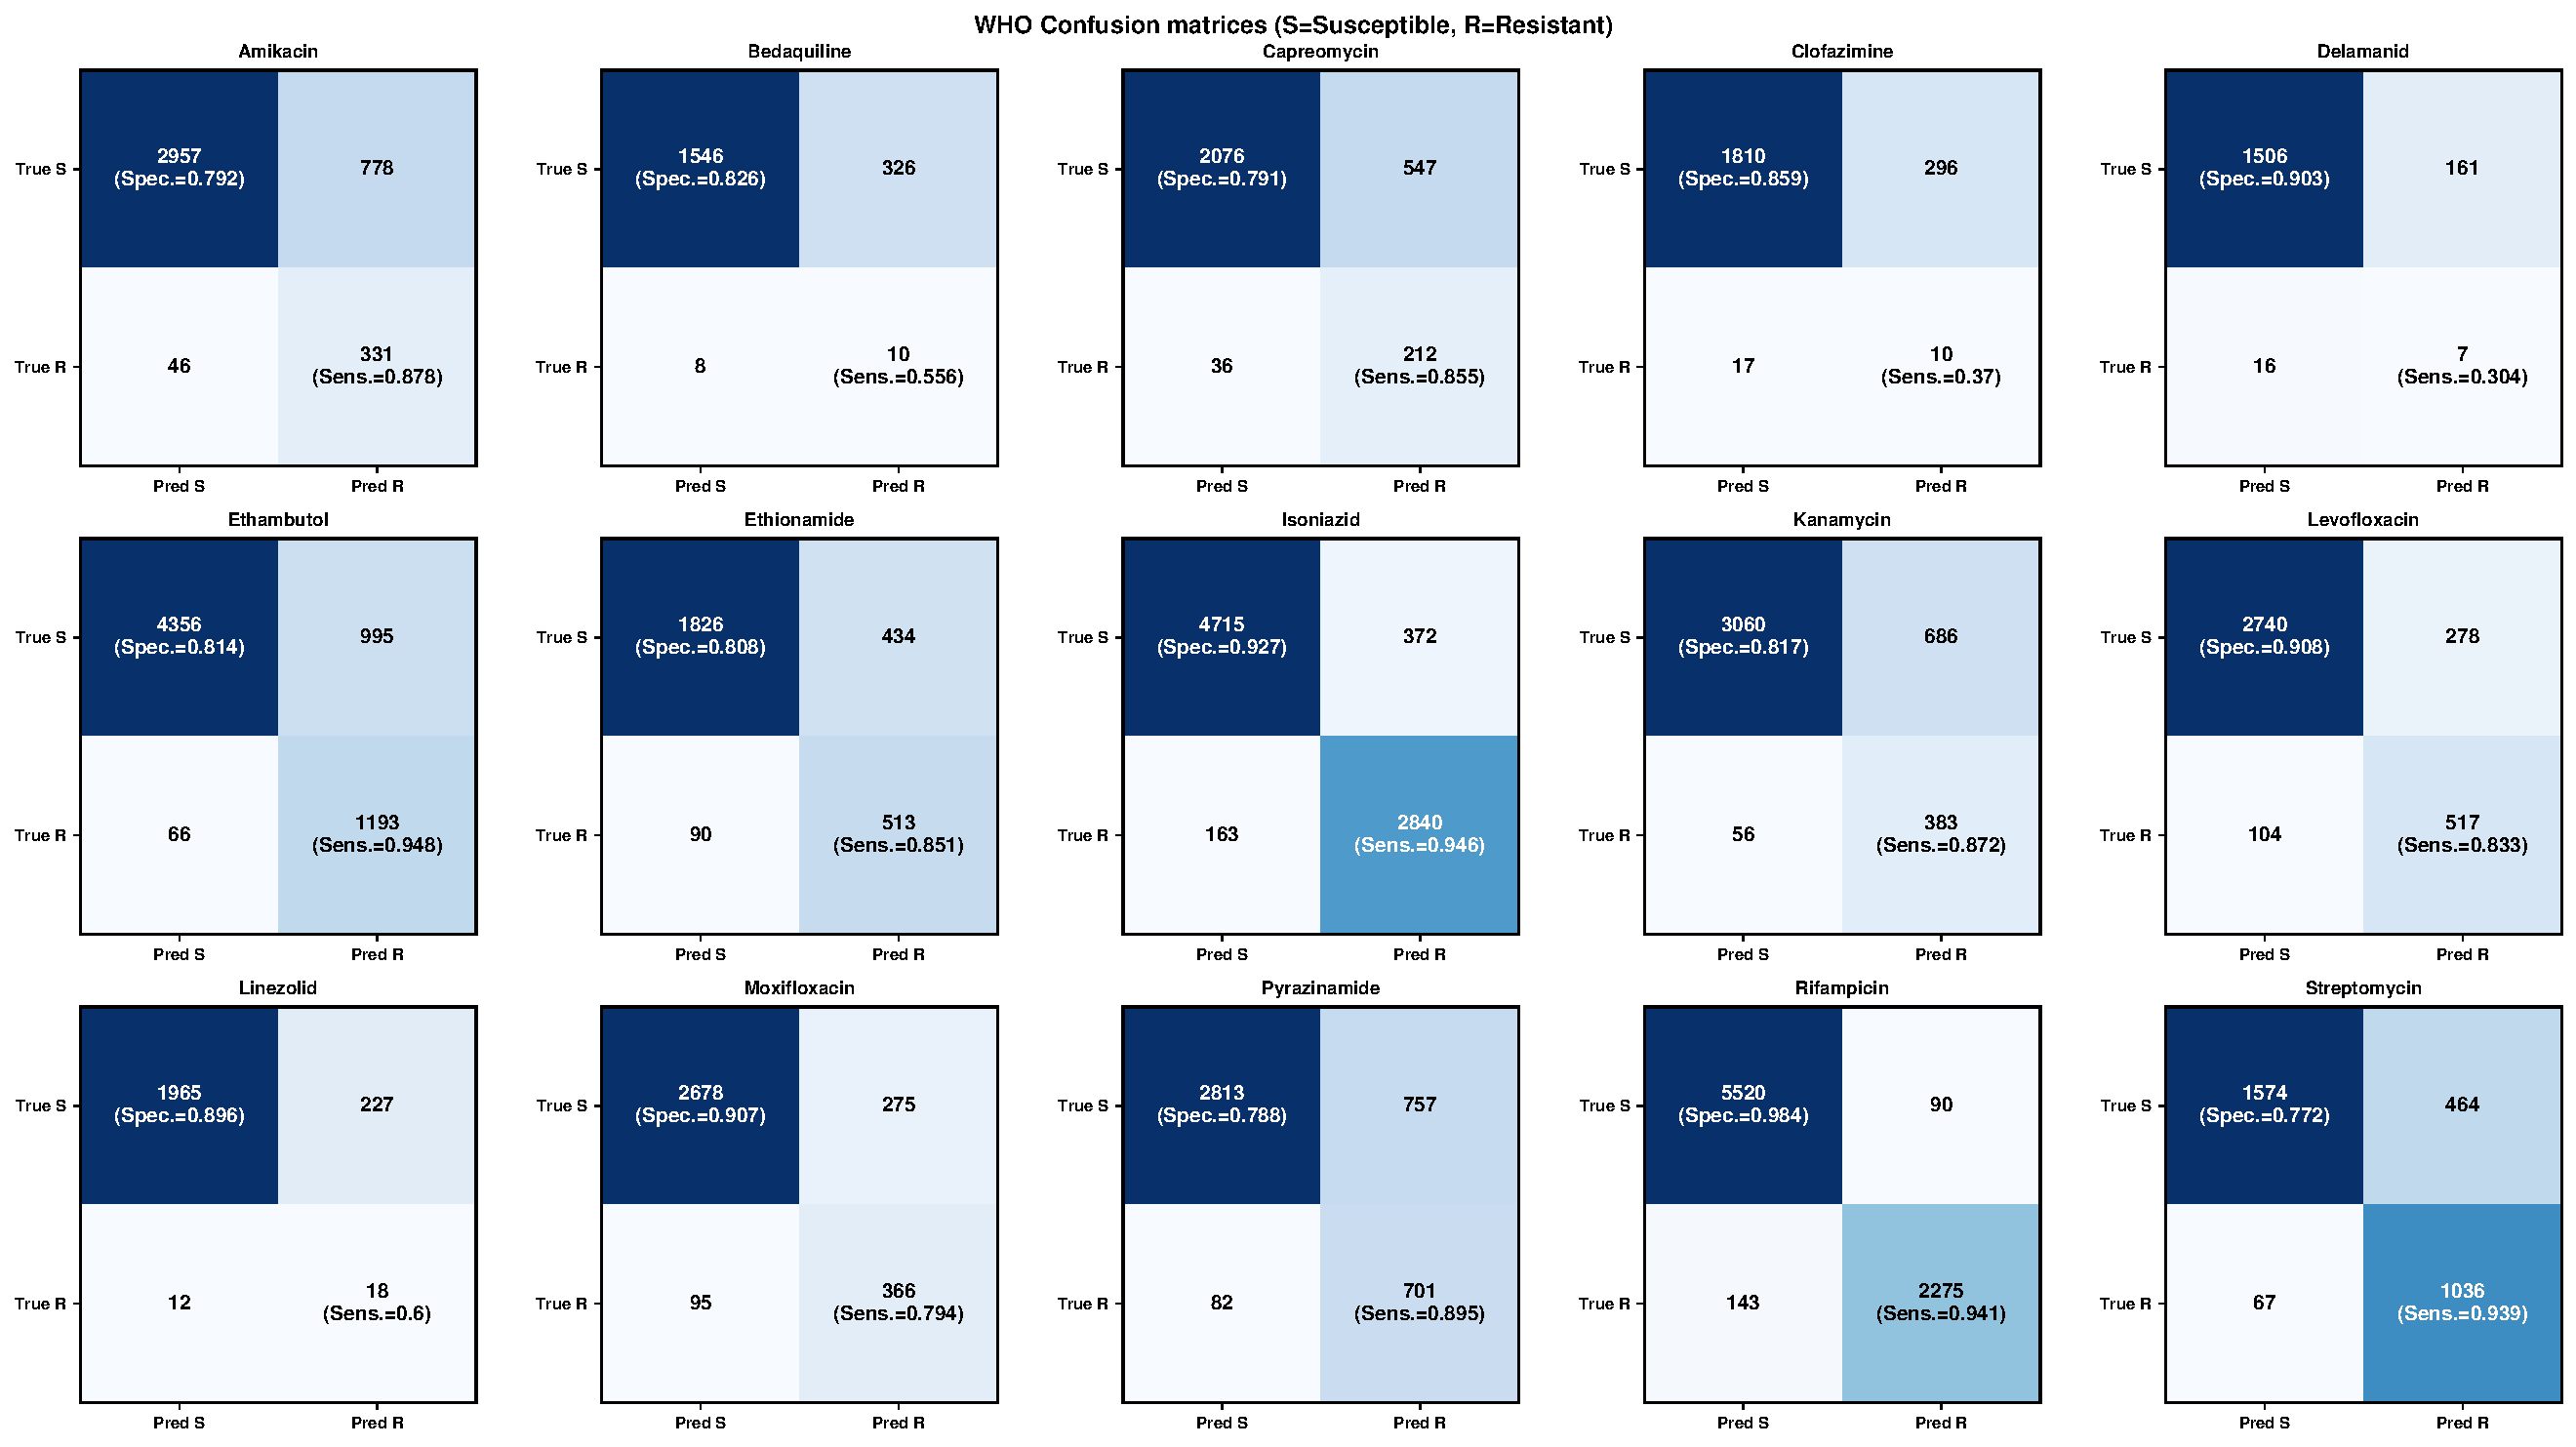
\includegraphics[width=\textwidth]{figures/who_confusion_matrices.pdf}
  \end{center}
  \caption{Confusion matrix for 15 drugs for the WHO snp catalogue}\label{fig:whocm}
\end{figure}

\begin{figure}[H]
  \begin{center}
    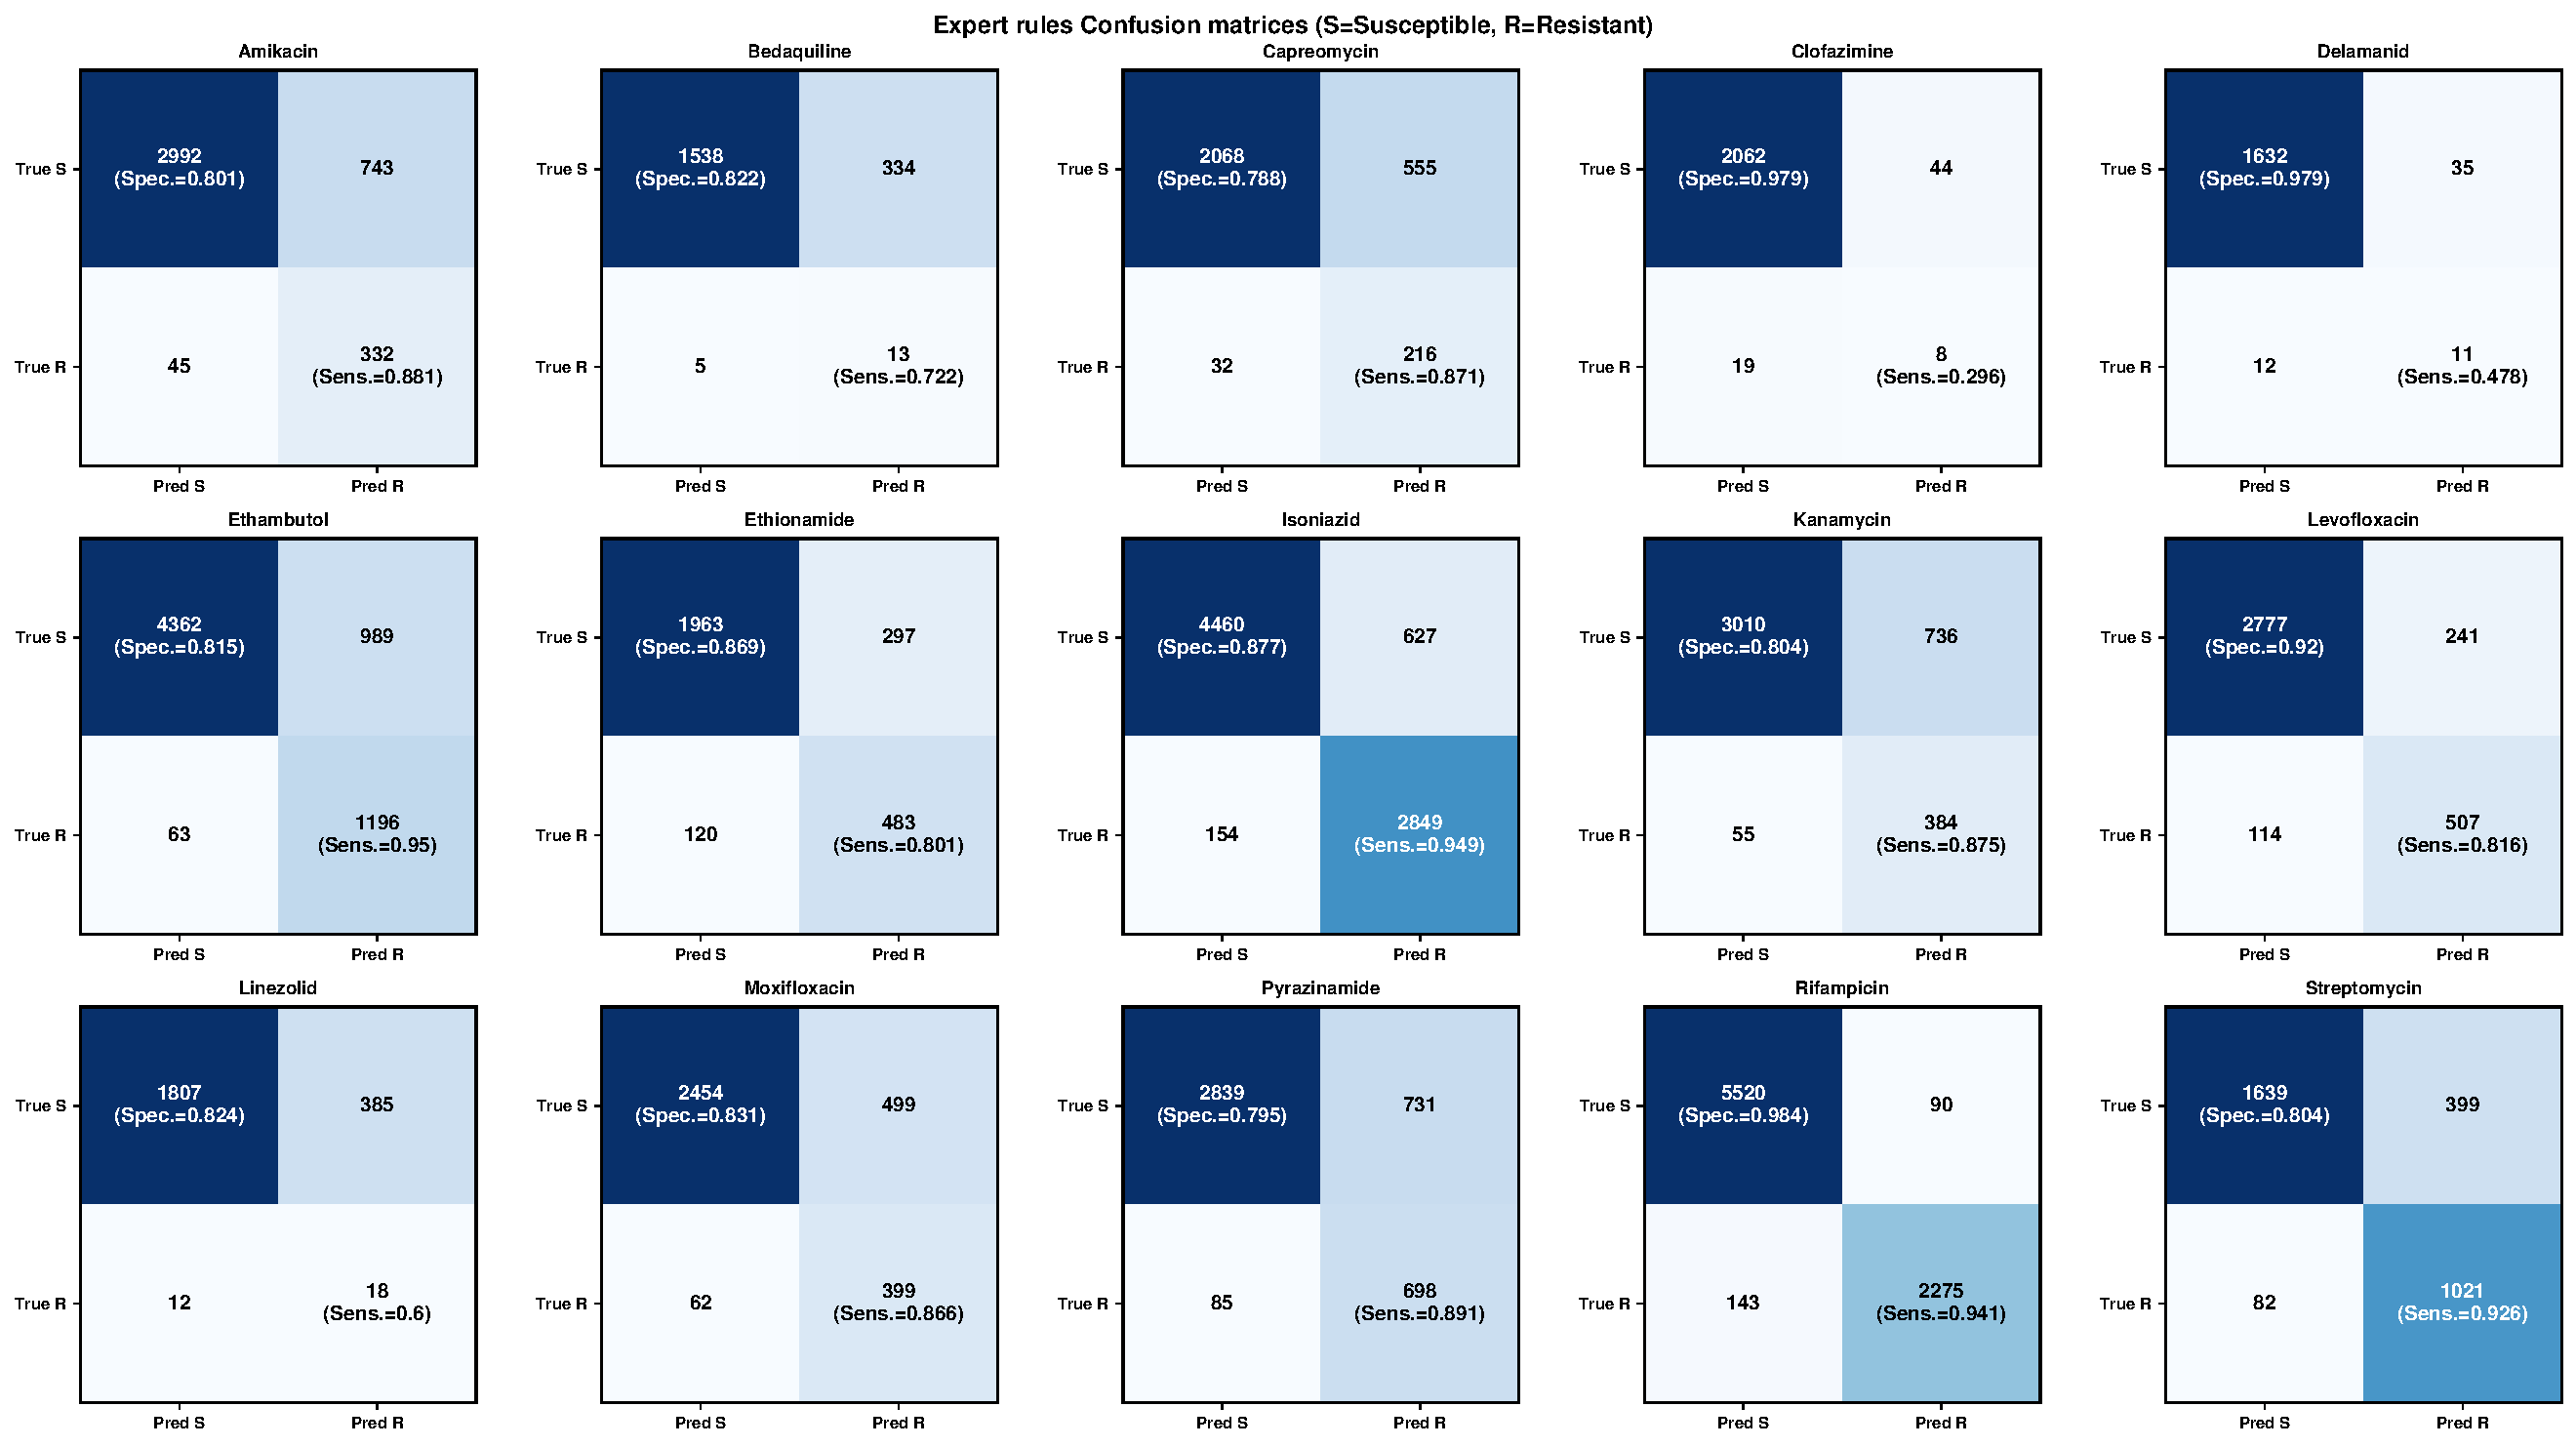
\includegraphics[width=\textwidth]{figures/expert_rules_confusion_matrices.pdf}
  \end{center}
  \caption{Confusion matrix for er+who catalogue.}\label{fig:ercm}
\end{figure}

\begin{figure}[H]
  \begin{center}
    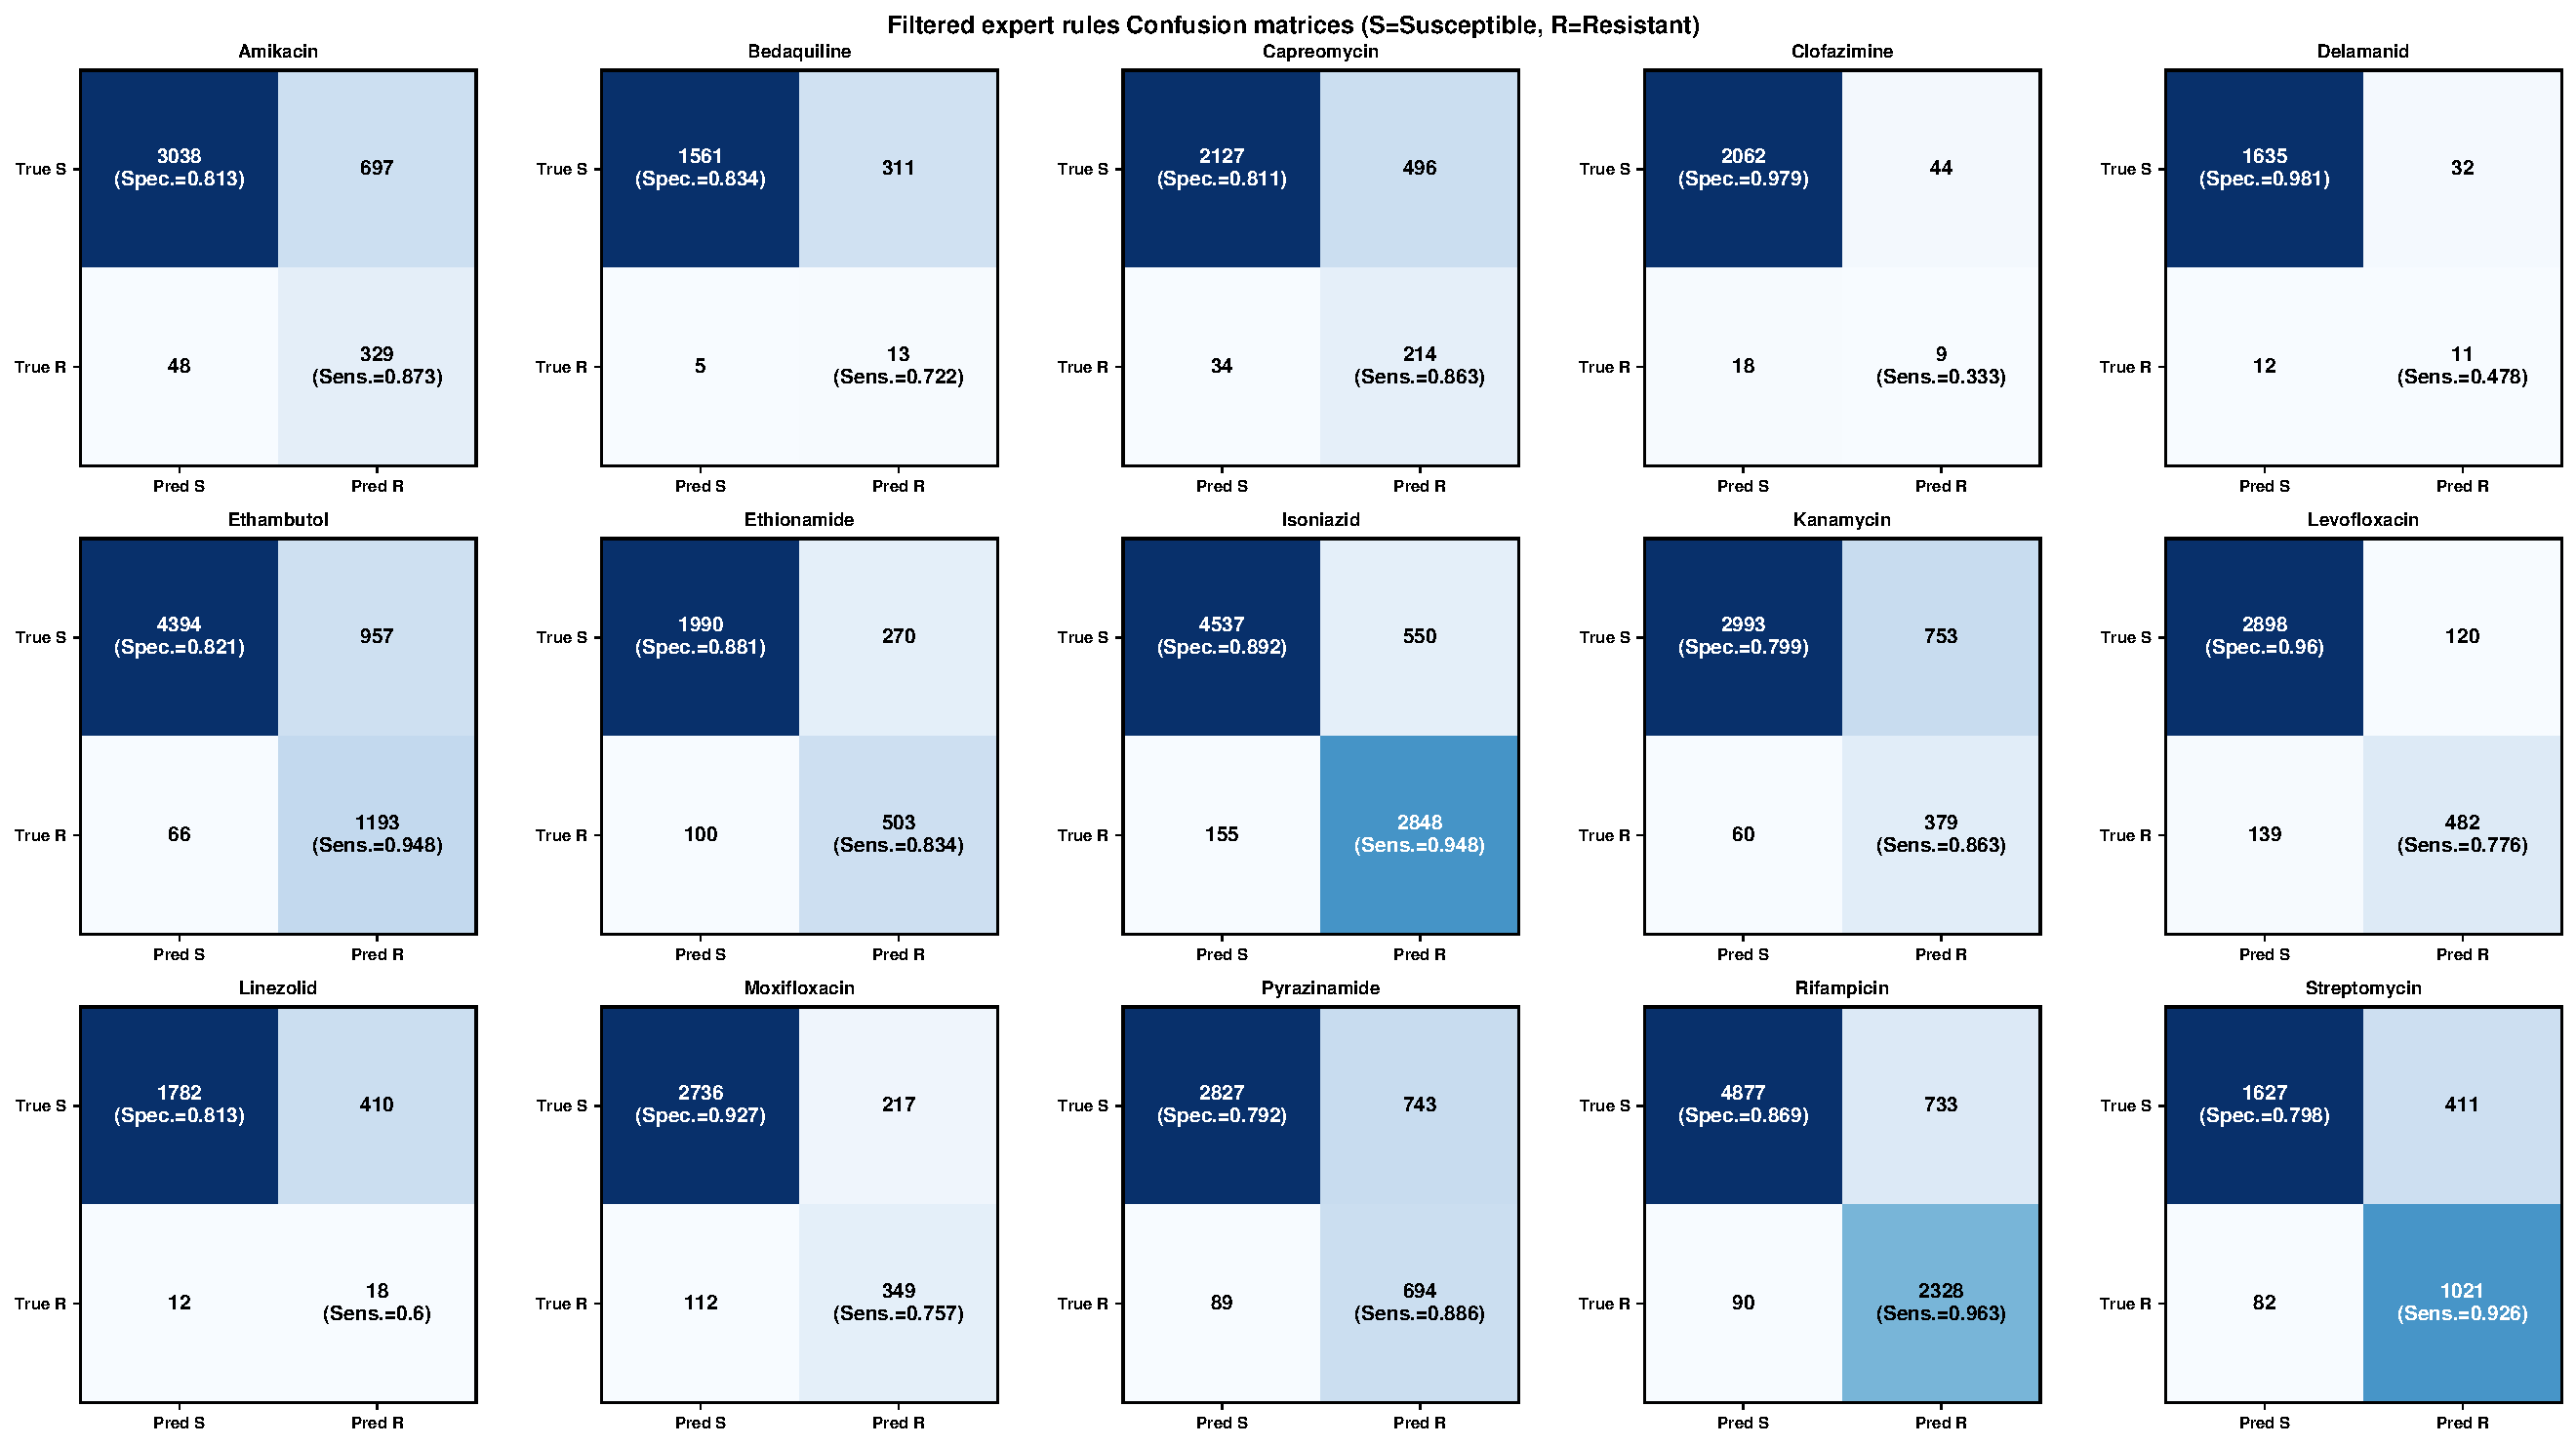
\includegraphics[width=\textwidth]{figures/filtered_expert_rules_confusion_matrices.pdf}
  \end{center}
  \caption{Confusion matrix for er+who+filt catalogue.}\label{fig:filtcm}
\end{figure}
\begin{figure}[H]
  \begin{center}
    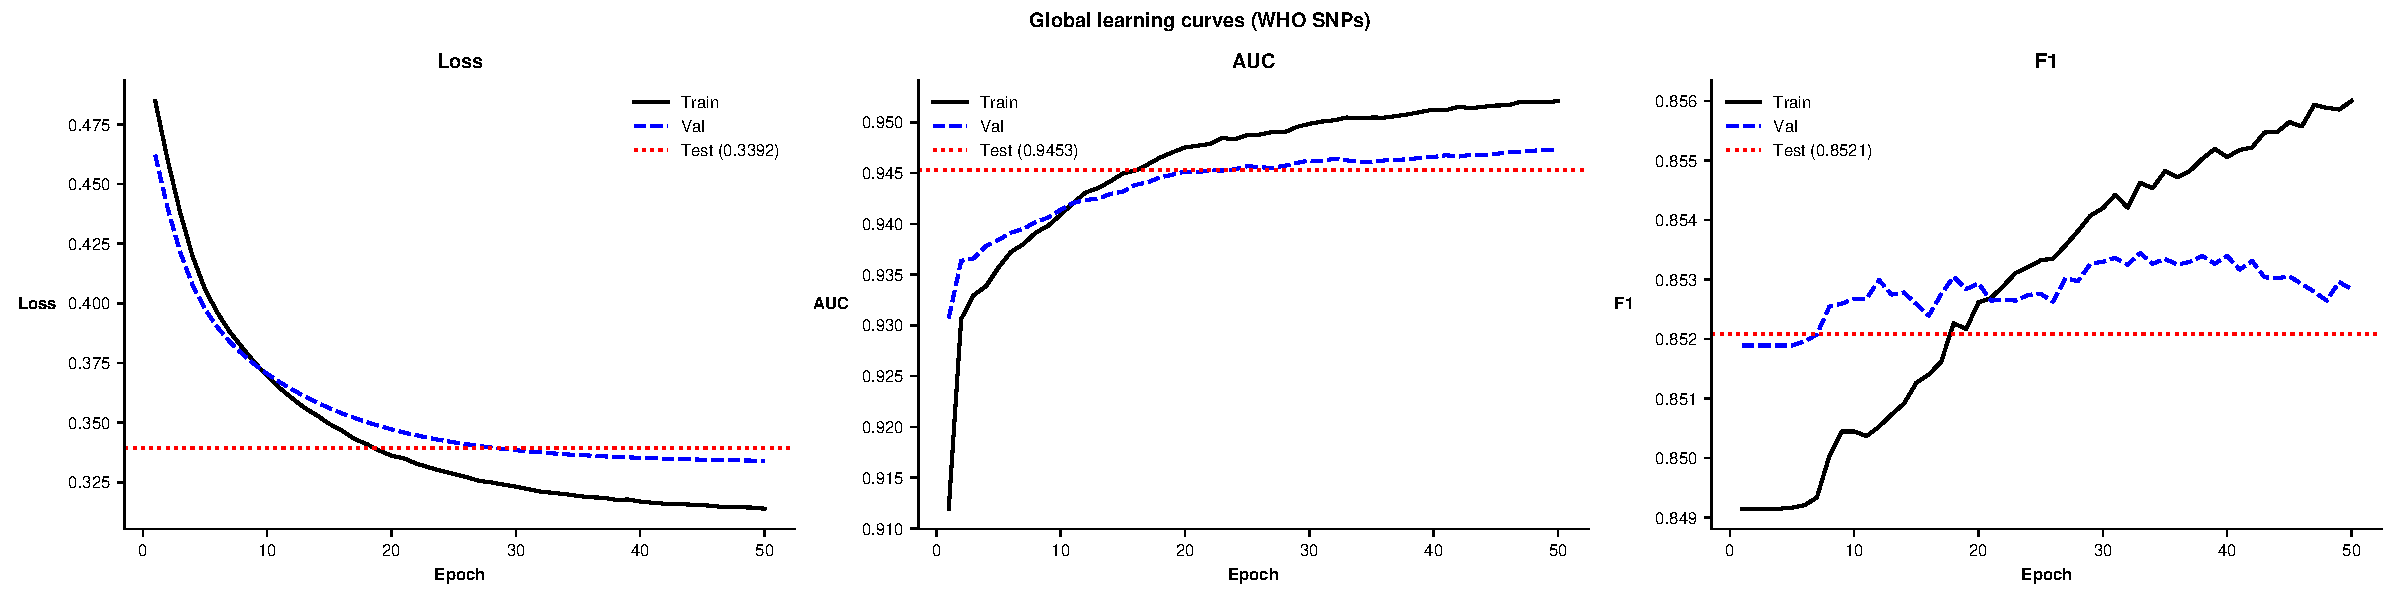
\includegraphics[width=\textwidth]{figures/who_learning_curves.pdf}
  \end{center}
  \caption{Global learning curves for who catalogue.}\label{fig:wholr}
\end{figure}

\begin{figure}[H]
  \begin{center}
    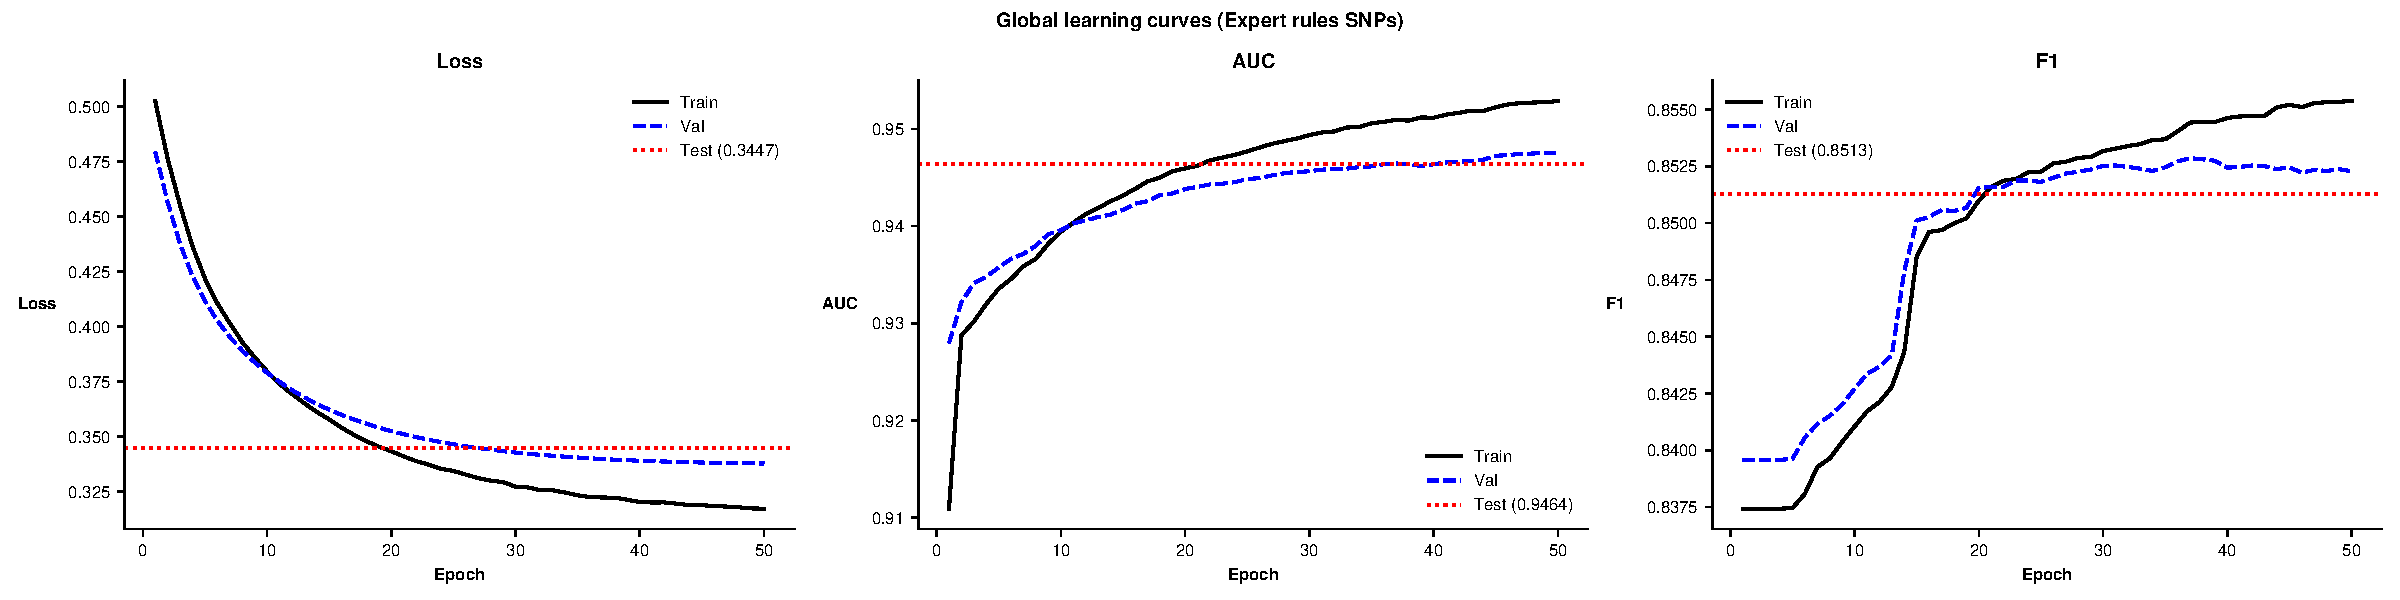
\includegraphics[width=\textwidth]{figures/expert_rules_learning_curves.pdf}
  \end{center}
  \caption{Global learning curves for er+who catalogue.}\label{fig:erlr}
\end{figure}

\begin{figure}[H]
  \begin{center}
    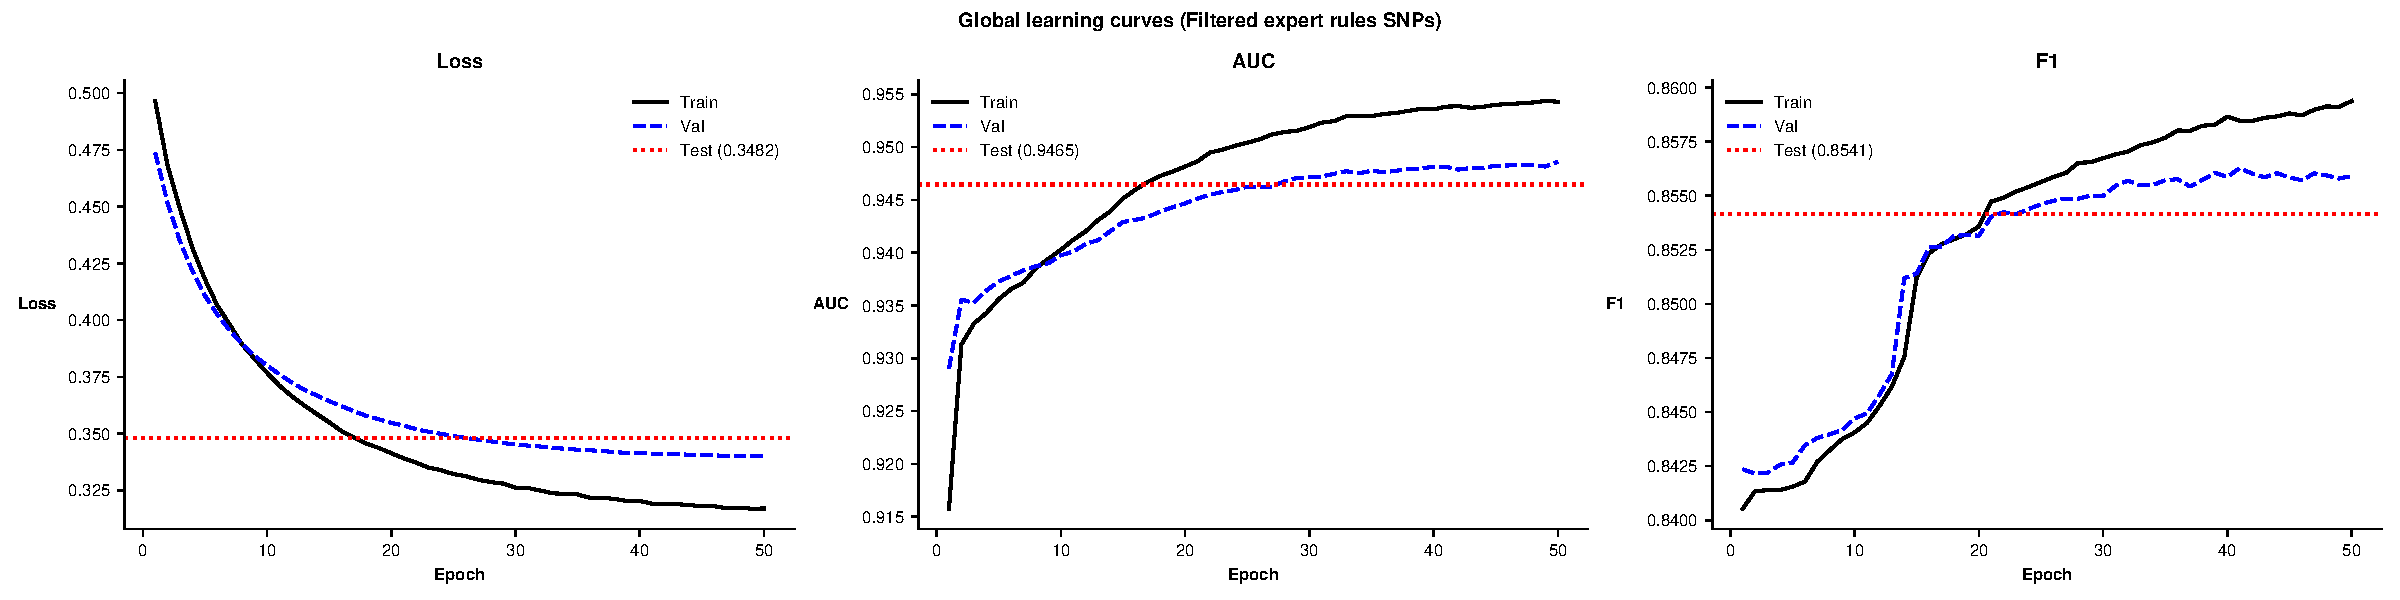
\includegraphics[width=\textwidth]{figures/filtered_expert_rules_learning_curves.pdf}
  \end{center}
  \caption{Global learning curves for er+who catalogue.}\label{fig:filerlr}
\end{figure}

% !TeX root = ../main.tex
% ============================================================
% REQUIRED PACKAGES -- add to your preamble if not present:
%   \usepackage{booktabs}
%   \usepackage{longtable}
%   \usepackage{array}
%   \usepackage{amsmath}
%   \usepackage{multirow}
% ============================================================
% --- BEGIN TABLE SNIPPET ---
\begingroup  % <- local scope; all settings below are restored after \endgroup
\small
\setlength{\tabcolsep}{4pt}
\renewcommand{\arraystretch}{1.15}

% Column widths scale automatically to the host document's \linewidth.
% Proportions: Drug 6% | Gene 12% | Variant 52% | FN 11% | R-missing 17%
\newlength{\colW}
\setlength{\colW}{\dimexpr\linewidth - 40pt\relax}% subtract 5 cols * 2 * 4pt tabcolsep

\newcommand{\tbsecrow}[1]{%
  \midrule[0.4pt]
  \multicolumn{5}{l}{\rule{0pt}{9pt}\textbf{\small #1}}\\[1pt]
}

\begin{longtable}{%
  >{\centering\arraybackslash}p{0.060\colW}%   Drug
  >{\raggedright\arraybackslash}p{0.120\colW}% Gene
  >{\raggedright\arraybackslash}p{0.520\colW}% Variant
  >{\centering\arraybackslash}p{0.110\colW}%   FN prevalence
  >{\centering\arraybackslash}p{0.170\colW}%   R samples missing variant
}

\caption{\textit{M.\,tuberculosis} variants surviving the false-negative
  filtering process, broken down by drug and locus. For every variant the
  table reports its false-negative (FN) prevalence and the proportion of
  resistant (R) samples in which the variant was absent.
  FN\,=\,false negative; R\,=\,resistant;
  ---\,=\,no relevant variant detected. Variants are written as
  \texttt{position\,REF}$\rightarrow$\texttt{ALT}.}
\label{tab:tb_variants}\\

\toprule
\textbf{Drug} & \textbf{Gene} & \textbf{Variant} &
\textbf{FN Prev.} & \textbf{R Samples Missing}\\
\midrule
\endfirsthead

\caption*{Table~\ref{tab:tb_variants} \textit{(continued)}}\\
\toprule
\textbf{Drug} & \textbf{Gene} & \textbf{Variant} &
\textbf{FN Prev.} & \textbf{R Samples Missing}\\
\midrule
\endhead

\midrule
\multicolumn{5}{r}{\small\textit{continued on next page}}\\
\endfoot

\bottomrule
\endlastfoot

% =======================================================
\tbsecrow{First-Line Drugs}
% =======================================================

\multirow{7}{*}{\textbf{RIF}} & \multirow{3}{*}{\textit{rpoB}} & 761110\,~\texttt{A}$\rightarrow$\texttt{T} & 89\% & 2\%\\*
 &  & 761139\,~\texttt{C}$\rightarrow$\texttt{G} & 100\% & 2\%\\*
 &  & 761155\,~\texttt{C}$\rightarrow$\texttt{T} & 97\% & 1\%\\*
\cmidrule(l){2-5}
 & PE\_PGRS6 & 624157\,~\texttt{T}$\rightarrow$\texttt{G} & 88\% & 2\%\\*
\cmidrule(l){2-5}
 & PPE54 & 3733405\,~\texttt{G}$\rightarrow$\texttt{A} & 73\% & 2\%\\*
\cmidrule(l){2-5}
 & \multirow{2}{*}{PPE60} & 3894503\,~\texttt{GGCC}$\rightarrow$\texttt{G} & 89\% & 2\%\\*
 &  & 3895400\,~\texttt{A}$\rightarrow$\texttt{C} & 71\% & 2\%\\
\midrule

\multirow{15}{*}{\textbf{INH}} & \multirow{10}{*}{\textit{katG}} & 2154016\,~\texttt{C}$\rightarrow$\texttt{T} & 90\% & 4\%\\*
 &  & 2154661\,~\texttt{C}$\rightarrow$\texttt{T} & 100\% & 4\%\\*
 &  & 2155168\,~\texttt{C}$\rightarrow$\texttt{G} & 100\% & 3\%\\*
 &  & 2155300\,~\texttt{G}$\rightarrow$\texttt{A} & 100\% & 4\%\\*
 &  & 2155417\,~\texttt{G}$\rightarrow$\texttt{C} & 100\% & 4\%\\*
 &  & 2155418\,~\texttt{G}$\rightarrow$\texttt{C} & 86\% & 4\%\\*
 &  & 2155546\,~\texttt{T}$\rightarrow$\texttt{C} & 80\% & 4\%\\*
 &  & 2155631\,~\texttt{A}$\rightarrow$\texttt{G} & 100\% & 4\%\\*
 &  & 2155687\,~\texttt{T}$\rightarrow$\texttt{C} & 88\% & 4\%\\*
 &  & 2155819\,~\texttt{T}$\rightarrow$\texttt{C} & 100\% & 4\%\\*
\cmidrule(l){2-5}
 & \textit{inhA} & 1674782\,~\texttt{T}$\rightarrow$\texttt{C} & 100\% & 4\%\\*
\cmidrule(l){2-5}
 & PE\_PGRS6 & 624157\,~\texttt{T}$\rightarrow$\texttt{G} & 88\% & 4\%\\*
\cmidrule(l){2-5}
 & \multirow{2}{*}{PPE54} & 3733405\,~\texttt{G}$\rightarrow$\texttt{A} & 73\% & 4\%\\*
 &  & 3733476\,~\texttt{A}$\rightarrow$\texttt{AG} & 37\% & 4\%\\*
\cmidrule(l){2-5}
 & PPE60 & 3894503\,~\texttt{GGCC}$\rightarrow$\texttt{G} & 89\% & 4\%\\
\midrule

\multirow{23}{*}{\textbf{ETH}} & \multirow{6}{*}{\textit{embB}} & 4247429\,~\texttt{A}$\rightarrow$\texttt{G} & 95\% & 2\%\\*
 &  & 4247431\,~\texttt{G}$\rightarrow$\texttt{C} & 80\% & 2\%\\*
 &  & 4247574\,~\texttt{A}$\rightarrow$\texttt{C} & 100\% & 2\%\\*
 &  & 4247730\,~\texttt{G}$\rightarrow$\texttt{C} & 80\% & 2\%\\*
 &  & 4247847\,~\texttt{A}$\rightarrow$\texttt{G} & 90\% & 2\%\\*
 &  & 4248003\,~\texttt{A}$\rightarrow$\texttt{G} & 92\% & 2\%\\*
\cmidrule(l){2-5}
 & \textit{embC} & 4241022\,~\texttt{C}$\rightarrow$\texttt{T} & 100\% & 2\%\\*
\cmidrule(l){2-5}
 & \textit{ubiA} & 4269271\,~\texttt{A}$\rightarrow$\texttt{G} & 100\% & 2\%\\*
\cmidrule(l){2-5}
 & PE\_PGRS4 & 336616\,~\texttt{C}$\rightarrow$\texttt{T} & 38\% & 2\%\\*
\cmidrule(l){2-5}
 & PE\_PGRS6 & 624157\,~\texttt{T}$\rightarrow$\texttt{G} & 88\% & 2\%\\*
\cmidrule(l){2-5}
 & \multirow{2}{*}{PE\_PGRS7} & 672683\,~\texttt{G}$\rightarrow$\texttt{A} & 80\% & 2\%\\*
 &  & 673482\,~\texttt{C}$\rightarrow$\texttt{T} & 100\% & 2\%\\*
\cmidrule(l){2-5}
 & \multirow{3}{*}{PE\_PGRS9} & 835953\,~\texttt{G}$\rightarrow$\texttt{A} & 32\% & 2\%\\*
 &  & 837826\,~\texttt{C}$\rightarrow$\texttt{T} & 36\% & 2\%\\*
 &  & 837943\,~\texttt{C}$\rightarrow$\texttt{A} & 42\% & 2\%\\*
\cmidrule(l){2-5}
 & PE\_PGRS19 & 1188873\,~\texttt{C}$\rightarrow$\texttt{G} & 100\% & 2\%\\*
\cmidrule(l){2-5}
 & PPE54 & 3733405\,~\texttt{G}$\rightarrow$\texttt{A} & 75\% & 2\%\\*
\cmidrule(l){2-5}
 & \multirow{4}{*}{PPE55} & 3744603\,~\texttt{T}$\rightarrow$\texttt{G} & 39\% & 2\%\\*
 &  & 3745906\,~\texttt{A}$\rightarrow$\texttt{G} & 65\% & 2\%\\*
 &  & 3747326\,~\texttt{C}$\rightarrow$\texttt{T} & 39\% & 2\%\\*
 &  & 3752124\,~\texttt{G}$\rightarrow$\texttt{A} & 40\% & 2\%\\*
\cmidrule(l){2-5}
 & \multirow{2}{*}{PPE60} & 3894484\,~\texttt{C}$\rightarrow$\texttt{T} & 62\% & 2\%\\*
 &  & 3894503\,~\texttt{GGCC}$\rightarrow$\texttt{G} & 89\% & 2\%\\
\midrule

\multirow{8}{*}{\textbf{PZA}} & \multirow{2}{*}{PE\_PGRS4} & 336635\,~\texttt{CCC\allowbreak GCC\allowbreak GTT\allowbreak G}$\rightarrow$\texttt{C} & 50\% & 3\%\\*
 &  & 338688\,~\texttt{C}$\rightarrow$\texttt{T} & 71\% & 3\%\\*
\cmidrule(l){2-5}
 & PE\_PGRS9 & 836018\,~\texttt{G}$\rightarrow$\texttt{A} & 80\% & 3\%\\*
\cmidrule(l){2-5}
 & \multirow{2}{*}{PPE54} & 3729592\,~\texttt{G}$\rightarrow$\texttt{A} & 100\% & 3\%\\*
 &  & 3734621\,~\texttt{C}$\rightarrow$\texttt{T} & 56\% & 3\%\\*
\cmidrule(l){2-5}
 & \multirow{2}{*}{PPE55} & 3752065\,~\texttt{A}$\rightarrow$\texttt{C} & 100\% & 3\%\\*
 &  & 3752419\,~\texttt{C}$\rightarrow$\texttt{G} & 62\% & 3\%\\*
\cmidrule(l){2-5}
 & PPE60 & 3894914\,~\texttt{C}$\rightarrow$\texttt{G} & 100\% & 3\%\\
\midrule

% =======================================================
\tbsecrow{Fluoroquinolones}
% =======================================================

\multirow{9}{*}{\textbf{CIP}} & \multirow{2}{*}{\textit{gyrA}} & 7570\,~\texttt{C}$\rightarrow$\texttt{T} & 91\% & 14\%\\*
 &  & 7582\,~\texttt{ACAG}$\rightarrow$\texttt{GCAC} & 97\% & 10\%\\*
\cmidrule(l){2-5}
 & \multirow{4}{*}{PE\_PGRS4} & 338648\,~\texttt{T}$\rightarrow$\texttt{G} & 73\% & 13\%\\*
 &  & 338669\,~\texttt{T}$\rightarrow$\texttt{C} & 59\% & 11\%\\*
 &  & 338682\,~\texttt{TCCC}$\rightarrow$\texttt{GGCG} & 74\% & 10\%\\*
 &  & 338690\,~\texttt{ATT}$\rightarrow$\texttt{GTC} & 64\% & 11\%\\*
\cmidrule(l){2-5}
 & PE\_PGRS19 & 1189137\,~\texttt{C}$\rightarrow$\texttt{CGC\allowbreak CGC\allowbreak CGG\allowbreak CCC\allowbreak CGC\allowbreak CGT\allowbreak T} & 74\% & 12\%\\*
\cmidrule(l){2-5}
 & PPE50 & 3501668\,~\texttt{G}$\rightarrow$\texttt{C} & 100\% & 13\%\\*
\cmidrule(l){2-5}
 & PPE54 & 3735033\,~\texttt{G}$\rightarrow$\texttt{A} & 80\% & 14\%\\
\midrule

\multirow{4}{*}{\textbf{LFX}} & \multirow{3}{*}{\textit{gyrA}} & 7570\,~\texttt{C}$\rightarrow$\texttt{T} & 70\% & 2\%\\*
 &  & 7572\,~\texttt{T}$\rightarrow$\texttt{C} & 100\% & 2\%\\*
 &  & 7582\,~\texttt{ACAG}$\rightarrow$\texttt{GCAC} & 100\% & 2\%\\*
\cmidrule(l){2-5}
 & PE\_PGRS33 & 2062066\,~\texttt{TCC\allowbreak GCC\allowbreak GGC\allowbreak GCC\allowbreak GCC\allowbreak GGC\allowbreak C}$\rightarrow$\texttt{T} & 20\% & 2\%\\
\midrule

\multirow{3}{*}{\textbf{MFX}} & \multirow{2}{*}{\textit{gyrA}} & 7570\,~\texttt{C}$\rightarrow$\texttt{T} & 40\% & 1\%\\*
 &  & 7582\,~\texttt{ACAG}$\rightarrow$\texttt{GCAC} & 44\% & 1\%\\*
\cmidrule(l){2-5}
 & PPE54 & 3733185\,~\texttt{G}$\rightarrow$\texttt{C} & 100\% & 1\%\\
\midrule

\multirow{12}{*}{\textbf{OFLX}} & \multirow{6}{*}{\textit{gyrA}} & 7570\,~\texttt{C}$\rightarrow$\texttt{T} & 88\% & 10\%\\*
 &  & 7572\,~\texttt{T}$\rightarrow$\texttt{C} & 91\% & 11\%\\*
 &  & 7581\,~\texttt{GACAG}$\rightarrow$\texttt{AACAC} & 94\% & 11\%\\*
 &  & 7582\,~\texttt{ACAG}$\rightarrow$\texttt{GCAC} & 94\% & 8\%\\*
 &  & 8639\,~\texttt{G}$\rightarrow$\texttt{A} & 78\% & 11\%\\*
 &  & 8955\,~\texttt{G}$\rightarrow$\texttt{C} & 100\% & 11\%\\*
\cmidrule(l){2-5}
 & \textit{gyrB} & 6608\,~\texttt{G}$\rightarrow$\texttt{C} & 69\% & 11\%\\*
\cmidrule(l){2-5}
 & \multirow{2}{*}{PE\_PGRS7} & 672738\,~\texttt{G}$\rightarrow$\texttt{CCGA} & 100\% & 11\%\\*
 &  & 675069\,~\texttt{C}$\rightarrow$\texttt{A} & 78\% & 11\%\\*
\cmidrule(l){2-5}
 & PPE54 & 3734189\,~\texttt{A}$\rightarrow$\texttt{T} & 59\% & 11\%\\*
\cmidrule(l){2-5}
 & PPE55 & 3747888\,~\texttt{T}$\rightarrow$\texttt{C} & 69\% & 11\%\\*
\cmidrule(l){2-5}
 & PPE68 & 4351991\,~\texttt{C}$\rightarrow$\texttt{A} & 100\% & 11\%\\
\midrule

% =======================================================
\tbsecrow{Diarylquinolines \& Riminophenazines}
% =======================================================

\textbf{BDQ} & --- & --- & --- & --- \\
\midrule

\multirow{2}{*}{\textbf{CFZ}} & PE\_PGRS9 & 836694\,~\texttt{ACC\allowbreak GGC\allowbreak GGG\allowbreak TTC\allowbreak GGC\allowbreak GAT\allowbreak ACC\allowbreak GAC\allowbreak GGG\allowbreak GGA\allowbreak GCC\allowbreak GGC\allowbreak GGT\allowbreak G}$\rightarrow$\texttt{A} & 20\% & 1\%\\*
\cmidrule(l){2-5}
 & PPE54 & 3734189\,~\texttt{A}$\rightarrow$\texttt{T} & 14\% & 1\%\\
\midrule

% =======================================================
\tbsecrow{Oxazolidinones \& Nitroimidazoles}
% =======================================================

\textbf{LZD} & --- & --- & --- & --- \\
\midrule

\multirow{1}{*}{\textbf{DLM}} & PPE54 & 3733795\,~\texttt{C}$\rightarrow$\texttt{T} & 14\% & 1\%\\
\midrule

% =======================================================
\tbsecrow{Injectable Agents (Aminoglycosides \& Cyclic Peptides)}
% =======================================================

\multirow{1}{*}{\textbf{AMK}} & \textit{rrs} & 1473246\,~\texttt{A}$\rightarrow$\texttt{G} & 100\% & 1\%\\
\midrule

\multirow{2}{*}{\textbf{KM}} & \textit{rrs} & 1473246\,~\texttt{A}$\rightarrow$\texttt{G} & 100\% & 2\%\\*
\cmidrule(l){2-5}
 & PPE68 & 4351991\,~\texttt{C}$\rightarrow$\texttt{A} & 60\% & 2\%\\
\midrule

\multirow{1}{*}{\textbf{CPM}} & \textit{rrs} & 1473246\,~\texttt{A}$\rightarrow$\texttt{G} & 90\% & 2\%\\
\midrule

\multirow{10}{*}{\textbf{SM}} & \textit{rpsL} & 781687\,~\texttt{A}$\rightarrow$\texttt{G} & 95\% & 8\%\\*
\cmidrule(l){2-5}
 & \textit{rrs} & 1473246\,~\texttt{A}$\rightarrow$\texttt{G} & 49\% & 7\%\\*
\cmidrule(l){2-5}
 & PE\_PGRS4 & 337482\,~\texttt{C}$\rightarrow$\texttt{T} & 62\% & 8\%\\*
\cmidrule(l){2-5}
 & PE\_PGRS33 & 2061424\,~\texttt{G}$\rightarrow$\texttt{A} & 62\% & 8\%\\*
\cmidrule(l){2-5}
 & PPE42 & 2935915\,~\texttt{C}$\rightarrow$\texttt{A} & 60\% & 8\%\\*
\cmidrule(l){2-5}
 & PPE51 & 3502457\,~\texttt{G}$\rightarrow$\texttt{A} & 58\% & 8\%\\*
\cmidrule(l){2-5}
 & \multirow{3}{*}{PPE54} & 3729613\,~\texttt{C}$\rightarrow$\texttt{T} & 66\% & 8\%\\*
 &  & 3732003\,~\texttt{CG}$\rightarrow$\texttt{C} & 67\% & 8\%\\*
 &  & 3732971\,~\texttt{G}$\rightarrow$\texttt{T} & 89\% & 8\%\\*
\cmidrule(l){2-5}
 & PPE55 & 3745863\,~\texttt{G}$\rightarrow$\texttt{A} & 68\% & 8\%\\
\midrule

% =======================================================
\tbsecrow{Second-Line Oral Agents}
% =======================================================

\multirow{8}{*}{\textbf{ETO}} & \multirow{2}{*}{\textit{inhA}} & 1674262\,~\texttt{A}$\rightarrow$\texttt{G} & 77\% & 5\%\\*
 &  & 1674481\,~\texttt{T}$\rightarrow$\texttt{G} & 100\% & 5\%\\*
\cmidrule(l){2-5}
 & PE\_PGRS19 & 1188514\,~\texttt{A}$\rightarrow$\texttt{G} & 86\% & 5\%\\*
\cmidrule(l){2-5}
 & PE\_PGRS33 & 2061315\,~\texttt{C}$\rightarrow$\texttt{A} & 77\% & 5\%\\*
\cmidrule(l){2-5}
 & PPE51 & 3502814\,~\texttt{G}$\rightarrow$\texttt{A} & 100\% & 5\%\\*
\cmidrule(l){2-5}
 & \multirow{3}{*}{PPE55} & 3748412\,~\texttt{G}$\rightarrow$\texttt{A} & 100\% & 5\%\\*
 &  & 3748936\,~\texttt{G}$\rightarrow$\texttt{A} & 77\% & 5\%\\*
 &  & 3752124\,~\texttt{G}$\rightarrow$\texttt{A} & 85\% & 5\%\\
\midrule

\textbf{PAS} & --- & --- & --- & --- \\
\midrule

\end{longtable}
\endgroup  % end local scope
% --- END TABLE SNIPPET ---

